\setcounter{section}{0}
\setcounter{propositions}{0}

\section{Analysis of Pairwise Loss for Spherical Embedding}
In this section, we provide proofs for the propositions presented in the paper
which provide some analytical understanding of our proposed objective function,
and the mechanism for subsequent pixel grouping mechanism.

\begin{propositions}
\label{theorem:ObjLowerBound_appendix}
For $n$ vectors $\{\x_1, \dots, \x_n\}$, the total intra-pixel similarity is
bounded as $\sum_{i\neq j} \x_i^T\x_j \ge -\sum_{i=1}^n  \Vert \x_i \Vert_2^2$.
In particular, for $n$ vectors on the hypersphere where $\Vert\x_i\Vert_2 = 1$,
we have $\sum_{i\neq j} \x_i^T\x_j \ge -n$.
\end{propositions}

\begin{proof}
  First note that $\Vert \x_1 + \dots + \x_n \Vert_2^2 \ge 0$.  We expand
  the square and collect all the cross terms so we have $\sum_{i} \x_i^T\x_i +
  \sum_{i\not=j}\x_i^T\x_j \ge 0$.  Therefore, $\sum_{i\not=j}\x_i^T\x_j \ge
  -\sum_{i=1}^n \Vert \x_i\Vert_2^2$.  When all the vectors are on the
  hyper-sphere, i.e. $\Vert \x_i\Vert_2 = 1$, then $\sum_{i\not=j}\x_i^T\x_j
  \ge -\sum_{i=1}^n \Vert \x_i\Vert_2^2= -n$. $\hfill\blacksquare$
\end{proof}


%\subsection{Proof of Proposition 2}
%We rewrite Proposition 2 as below.

%\begin{equation}
%\small
%\begin{split}
%\ell = \sum_{k=1}^M  \sum_{i,j=1}^{N_k} \frac{w^k_i w^k_j}{N_k} \Big( \1_{\{y_i=y_j\}}(1-s_{ij})
% &+ \1_{\{y_i\not=y_j\}} [s_{ij}-\alpha]_{+} \Big)
%\end{split}
%\label{eq:obj}
%\end{equation}

\begin{propositions}
\label{lemma:max_margin_appendix}
If $n$ vectors $\{\x_1, \dots, \x_n\}$ are distributed on a 2-sphere (i.e.
$\x_i \in \RB^3$ with $\Vert\x_i\Vert_2 = 1, \forall i=1\dots n$) then the
similarity between any pair is lower-bounded by $s_{ij} \geq
1-\Big(\frac{2\pi}{\sqrt{3}n} \Big)$. Therefore, choosing the parameter
$\alpha$ in the maximum margin term in objective function to be less
than
$1-\Big(\frac{2\pi}{\sqrt{3}n} \Big)$ results in positive loss even for
a perfect embedding of $n$ instances.
\end{propositions}

We treat all the $n$ vectors as representatives of $n$ different instances in
the image and seek to minimize pairwise similarity, or equivalently maximize
pairwise distance (referred to as Tammes's problem, or the hard-spheres
problem~\cite{saff1997distributing}).

\begin{proof}
Let $d  = \max\limits_{\{\x_i\}} \min\limits_{i\not=j}\Vert \x_i-\x_j\Vert_2$
be the distance between the closest point pair of the optimally distributed
points.  Asymptotic results in~\cite{habicht1951lagerung} show that, for some
constant $C>0$,
\begin{equation}
  \Big(\frac{8\pi}{\sqrt{3}n}\Big)^{\frac{1}{2}} -Cn^{-\frac{2}{3}} \le d \le \Big( \frac{8\pi}{\sqrt{3}n} \Big)^{\frac{1}{2}}
\end{equation}
Since $\Vert \x_i-\x_j\Vert_2^2=2-2\x_i^T \x_j$, we can rewrite this bound in
terms of the similarity
$s_{ij} = \frac{1}{2}\left(1 + \frac{\x_i^T\x_j}{\Vert\x_i\Vert_2 \Vert\x_j\Vert_2}\right)$,
so that for any $i \not= j$:
\begin{equation}
1- \Big( \frac{2\pi}{\sqrt{3}N} \Big) \le s_{ij} \le  1- \frac{1}{4} \Bigg( \Big(\frac{8\pi}{\sqrt{3}N}\Big)^{\frac{1}{2}} -CN^{-\frac{2}{3}}\Bigg)^2
\end{equation}
Therefore, choosing $\alpha \leq 1- \Big( \frac{2\pi}{\sqrt{3}N} \Big)$,
guarantees that $[s_{ij}-\alpha]_{+}\geq 0$ for some pair $i \not= j$. Choosing
$\alpha > 1- \frac{1}{4} \Bigg( \Big(\frac{8\pi}{\sqrt{3}N}\Big)^{\frac{1}{2}}
-CN^{-\frac{2}{3}}\Bigg)^2$, guarantees the existence of an embedding with
$[s_{ij}-\alpha]_{+}=0$.
$\hfill\blacksquare$
\end{proof}

\begin{figure*}[t]
\centering
   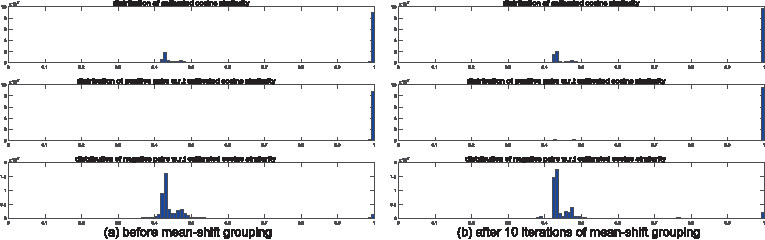
\includegraphics[width=1\linewidth]{pixel_pair_distr}
   \caption{Distribution of calibrated cosine similarity between pairs of pixels.
   After 10 iterations of mean-shift grouping.  Margin is 0.5 for negative
   pairs.  From the figures, we believe that the mean shift grouping mechanism
   forces learning to focus on those pixel pairs that will not be corrected by
   mean shift grouping itself if running offline, and thus pushing down to
   parameters in the the deep neural network to learn how to correct them
   during training.
   }
\label{fig:pixel_pair_distr}
\end{figure*}


\section{Details of Recurrent Mean Shift Grouping }

There are two commonly used multivariate kernels in mean shift algorithm.  The
first, Epanechnikov kernel~\cite{epanechnikov1969non,cheng1995mean}, has the
following profile
\begin{equation}
K_E(\x)=
\begin{cases}
    \frac{1}{2} c_d^{-1} (d+2) (1-\Vert\x \Vert_2^2),& \text{if } \Vert\x\Vert_2\le 1\\
    0,              & \text{otherwise}
\end{cases}
\end{equation}
where $c_d$ is the volume of the unit $d$-dimensional sphere. The standard
mean-shift algorithm computes the gradient of the kernel density estimate
given by
\[
p(\x) = \frac{1}{N} \sum_{i=1}^N K_E(\frac{\x - \x_i}{b})
\]
and identifies modes (local maxima) where $\nabla p(\x)= 0$. The scale
parameter $b$ is known as the kernel bandwidth and determines the
smoothness of the estimator.  The gradient of $p(\x)$ can be elegantly computed
as the difference between $\x$ and the mean of all data points with $\Vert \x -
\x_i \Vert \leq b$, hence the name ``mean-shift'' for performing gradient
ascent.

Since the Epanechnikov profile is not differentiable at the boundary, we
use the squared exponential kernel adapted to vectors on the sphere:
\begin{equation}
\begin{split}
K(\x,\x_i) & \propto \exp( \delta^2 \x^T \x_i ) \\
\end{split}
\end{equation}
which can be viewed as a natural extension of the Gaussian to spherical data
(known as the von Mises Fisher (vMF)
distribution~\cite{fisher1953dispersion,banerjee2005clustering,mardia2009directional,kobayashi2010mises}).
In our experiments we set the bandwidth $\delta$ based on the margin $\alpha$
so that $\frac{1}{\delta}=\frac{1-\alpha}{3}$.

Our proposed algorithm also differs from the standard mean-shift clustering
(i.e., ~\cite{comaniciu1999mean}) in that rather than performing gradient
ascent on a fixed kernel density estimate $p(\x)$, at every iteration we
alternate between updating the embedding vectors $\{\x_i\}$ using gradient
ascent on $p(\x)$ and re-estimating the density $p(\x)$ for the updated
vectors.  This approach is termed Gaussian Blurring Mean Shift (GBMS) in
~\cite{carreira2008generalised} and has converge rate guarantees for
data which starts in compact clusters.

In the paper we visualized embedding vectors after GBMS for specific
examples.  Figure~\ref{fig:pixel_pair_distr} shows aggregate statistics over a
collection of images (in the experiment of instance segmentation).
We plot the distribution of pairwise similarities for
positive and negative pairs during forward propagation through 10 iterations.
We can observe that the mean shift module produces sharper distributions,
driving the similarity between positive pairs to 1 making it trivial to
identify instances.

\subsection{Gradient Calculation for Recurrent Mean Shift}

To backpropagate gradients through an iteration of GBMS, we break the
calculation into a sequence of steps below where we assume the vectors
in the data matrix $X$ have already been normalized to unit length.
\begin{equation}\small
\begin{split}
&\colorboxed{red}{
\begin{split}
\S = & \X^T\X \\
\end{split}
}\\
&\colorboxed{blue}{
\begin{split}
\K = & \exp(\delta^2 \S) \\
\end{split}
}, \\
&\colorboxed{green}{
\begin{split}
{\bf d} = & \K^T\1 \\
\end{split}
}\\
& \colorboxed{black}{
\begin{split}
\q = & {\bf d}^{-1} \\
\end{split}
}\\
&\colorboxed{orange}{
\begin{split}
{\bf P} = (1-\eta)\I + \eta\K \diag(\q)\\
\end{split}
}\\
&\colorboxed{cyan}{
\begin{split}
\Y = & \X{\bf P} \\
\end{split}
}\\
\end{split}
\label{eq:GBMS_matrix_form}
\end{equation}
where $\Y$  is the updated data after one iteration which is subsequently
renormalized to project back onto the sphere.  Let $\ell$ denote the loss
and $\odot$ denote element-wise product. Backpropagation gradients are
then given by:
\begin{equation}\small
\begin{split}
&\colorboxed{red}{
\begin{split}
&\frac{\partial \ell}{\partial \X} =  2\X \frac{\partial \ell}{\partial \S} \\
\end{split}
}\\
&\colorboxed{blue}{
\begin{split}
&\frac{\partial \ell}{\partial\S} =  \delta^2\exp(\delta^2\S) \odot \frac{\partial \ell}{\partial\K} \\
&\frac{\partial \ell}{\partial\delta} =  2\delta \sum_{ij} \Big( (s_{ij}) \odot \exp(\delta^2 s_{ij}) \odot \frac{\partial \ell}{\partial {k_{ij}}} \Big)\\
\end{split}
}\\
&\colorboxed{green}{
\begin{split}
&\frac{\partial \ell}{\partial{\bf K}} =  \1 \Big( \frac{\partial \ell}{\partial {\bf d}} \Big)^T \\
\end{split}
}\\
&\colorboxed{black}{
\begin{split}
&\frac{\partial \ell}{\partial{\bf d}} =  \frac{\partial \ell}{\partial{\bf q}} \odot (-{\bf d}^{-2}) \\
\end{split}
}\\
&\colorboxed{orange}{
\begin{split}
&\frac{\partial \ell}{\partial{\bf K}} =  \eta\Big(\frac{\partial \ell}{\partial{\bf P}}\Big) (\q\1^T)\\
&\frac{\partial \ell}{\partial{\bf q}} =  \eta\Big(\frac{\partial \ell}{\partial{\bf P}}\Big)^T \K\1 \\
\end{split}
}\\
&\colorboxed{cyan}{
\begin{split}
&\frac{\partial \ell}{\partial{\bf X}} =  \frac{\partial \ell}{\partial{\bf Y}} {\bf P}^T \\
&\frac{\partial \ell}{\partial{\bf P}} =  \X^T \frac{\partial \ell}{\partial{\bf Y}} \\
\end{split}
}
\end{split}
\end{equation}



%\subsection{Stability of Mean Shift Gradients}
%
%Note that, when reformulating mean shift in matrix form, we can construct a
%transition matrix ${\bf P} \in \RB^{N\times N}$ (see
%Equation~\ref{eq:GBMS_matrix_form} by setting $\eta=1$).  Update of 64
%iterations results into the following tweaked data points:
%\begin{equation}
%\begin{split}
%\tilde \x \leftarrow & \x {\bf P}\cdot\cdot\cdot\cdot{\bf P} \\
%    \leftarrow & \x {\bf P}^{K}
%\end{split}
%\end{equation}
%where $K=64$ denotes the iteration number.
%
%[the Jacobian is ... we can show that the eigenvalues go to .. so no
%vanishing gradients]
%
%While it is difficult to analyze directly GBMS in the supervised scenario, we
%carry out this series of simulation experiments to help understand the gradient
%through mean shift grouping module.

\subsection{Toy Example of Mean Shift Backpropagation}
In the paper we show examples of the gradient vectors backpropagated through
recurrent mean shift to the initial embedding space. Backpropagation through
this fixed model modulates the loss on the learned embedding, increasing the
gradient for initial embedding vectors whose instance membership is ambiguous
and decreasing the gradient for embedding vectors that will be correctly
resolved by the recurrent grouping phase.

Figure \ref{fig:simulation_trajectory} shows a toy example highlighting the difference
between supervised and unsupervised clustering.  We generate  a set of 1-D data
points drawn from three Gaussian distributions with mean and standard deviation
as $(\mu=3, \sigma=0.2)$, $(\mu=4, \sigma=0.3)$ and $(\mu=5, \sigma=0.1)$,
respectively, as shown in Figure \ref{fig:simulation_trajectory} (a).
We use mean squared error for the loss with a fixed linear
regressor $y_i = 0.5*x_i-0.5$ and fixed target labels. The optimal embedding
would set $x_i=3$ if $y_i=1$, and $x_i=5$ if $y_i=2$. We perform 30 gradient
updates of the embedding vectors $x_i \leftarrow x_i - \alpha \nabla_{x_i}
\ell$ with a step size $\alpha$ as 0.1.
We analyze the behavior of Gaussian Blurring Mean Shift (GBMS) with bandwidth as $0.2$.

If running GBMS for unsupervised clustering on these data with the default setting (bandwidth is 0.2),
we can see they are grouped into three piles,
as shown in Figure \ref{fig:simulation_trajectory} (b).
If updating the data using gradient descent without GBMS inserted,
we end up with three visible clusters even though the data move towards the ideal embedding in terms of classification.
Figure \ref{fig:simulation_trajectory} (c) and (d) depict the trajectories of 100 random data points during the 30 updates and the final result, respectively.


Now we insert the GBMS module to update these data with different loops,
and compare how this effects the performance.
We show the updated data distributions and those after five loops of GBMS grouping in column (e) and (f) of Figure~\ref{fig:simulation_trajectory},
respectively.
We notice that, with GBMS,
all the data are grouped into two clusters;
while with GBMS grouping they become more compact and are located exactly on
the ``ideal spot'' for mapping into label space (i.e. 3 and 5) and achieving
zero loss.
On the other hand,
we also observe that, even though these settings incorporates different number of GBMS loops,
they achieve similar visual results in terms of clustering the data.
To dive into the subtle difference,
we randomly select 100 data and depict their trajectories in column (g) and (h)
of Figure~\ref{fig:simulation_trajectory},
using a single loss on top of the last GBMS loop or multiple losses over every GBMS loops,
respectively.
We have the following observations:
\begin{enumerate}
  \item By comparing with Figure~\ref{fig:simulation_trajectory} (c),
    which depicts update trajectories without GBMS,
    GBMS module provides larger gradient to update those data further from their ``ideal spot'' under both scenarios.
  \item From (g),
    we can see the final data are not updated into tight groups.
    This is because that the updating mechanism only sees data after (some loops of) GBMS,
    and knows that these data will be clustered into tight groups through GBMS.
  \item A single loss with more loops of GBMS provides greater gradient than that with fewer loops to update data, as seen in (g).
  \item With more losses over every loops of GBMS,
    the gradients become even larger that the data are grouped more tightly and more quickly.
    This is because that the updating mechanism also incorporates the gradients from the loss over the original data,
    along with those through these loops of GBMS.
\end{enumerate}

To summarize,
our GBMS based recurrent grouping module indeed provides meaningful gradient during training with back-propagation.
With the convergent dynamics of GBMS,
our grouping module becomes especially more powerful in learning to group data with suitable supervision.

%To summarize, we observe that
%\begin{enumerate}
%  \item Embedding mean shift module in the supervised regression system helps
%  learning. Note that the gradients w.r.t data points can be transmitted down
%  to the deep neural networks if existing.
%  \item GBMS performs much faster than the standard mean shift w.r.t clustering
%  data.  Moreover, GBMS seems to help than the standard mean shift in the
%  supervised scenario.
%  \item The transition matrix used in standard mean shift seems to constrain
%  data and prevent a better updating mechanism (suppose the data points are
%  dragged each other), as seen in Figure~\ref{fig:simulation} (e) that data
%  points are off the ``ideal spot''.  But GBMS detects the ``ideal spot'' and
%  place data around there (see Figure~\ref{fig:simulation} (h)).  We conjecture
%  the reason is that transition matrix is being updated simultaneously during
%  back-propagation, in which way the constraints among data points are getting
%  loose during updating.
%\end{enumerate}

%\begin{figure*}[t]
%\centering
%   \includegraphics[width=1\linewidth]{simulation_results}
%   \caption{Simulation experiment with generated 1D embedding and binary labels:
%   Class-1 and 2 are highlighted by red and blue color, respectively.  A fixed
%   regressor is used for supervised learning, mapping data from $x$ to the
%   label space for classification.  Over the original data, loss is high for
%   points in the middle cluster near the decision boundary after grouping.
%   Back-propagating the loss to shift the data points to better fit the
%   regressor (either standard version or Gaussian Blurring Mean Shift, GBMS for
%   short) modifies the embedding to fix these ambiguous points while ignoring
%   points far from the decision boundary.}
%\label{fig:simulation}
%\end{figure*}



\begin{figure*}[t]
\centering
   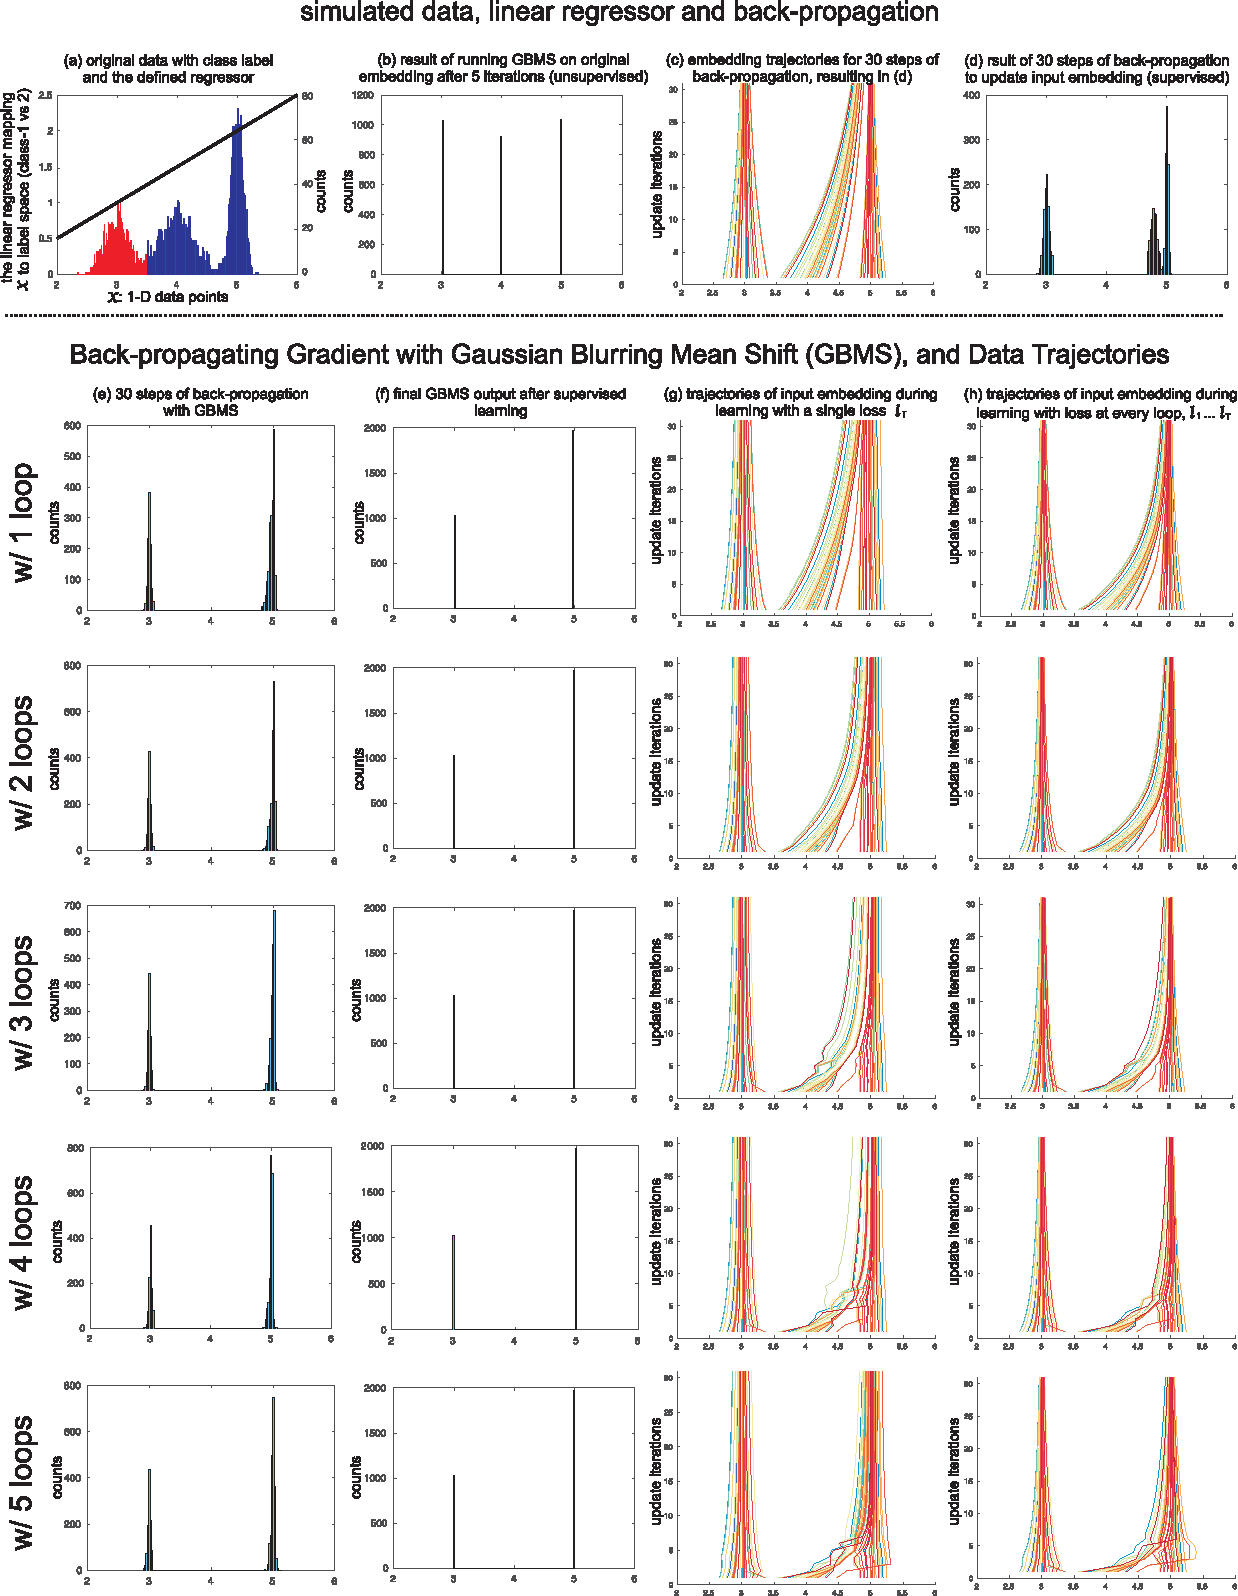
\includegraphics[width=0.9\linewidth]{simulation_random_trajectory}%{simulation_results_trajectory}
   \caption{
   Trajectory of updating data using back-propagation without mean shift module (top row),
   and with the Gaussian Blurring Mean Shift (GBMS).
   To compare the results,
   we vary the number of GBMS loops in the grouping module,
   and use either a single loss at the final GBMS loop or multiple losses on all GBMS loops.
   All the configurations can shift data towards the ``ideal spots'' (3 or 5 depending on the label) in terms of the fixed regressor.
   }
\label{fig:simulation_trajectory}
\end{figure*}

\section{Additional Boundary Detection Results}

We show additional boundary detection results\footnote{Paper with high-resolution figures can be found at the
\href{http://www.ics.uci.edu/~skong2/SMMMSG.html}{Project Page}.} on BSDS500
dataset~\cite{arbelaez2011contour} based on our model in Figure
\ref{fig:boundary_show_appendix_part1},
%\ref{fig:boundary_show_appendix_part2},
\ref{fig:boundary_show_appendix_part3},
\ref{fig:boundary_show_appendix_part4}
and \ref{fig:boundary_show_appendix_part5}.
Specifically, besides showing the boundary detection result, we also show
3-dimensional pixel embeddings as RGB images before and after fine-tuning using
logistic loss.  From the consistent colors, we can see (1) our model
essentially carries out binary classification even using the pixel pair
embedding loss; (2) after fine-tuning with logistic loss, our model captures
also boundary orientation and signed distance to the boundary.  Figure
\ref{fig:demo_test_boundary} highlights this observation for an example image
containing round objects.  By zooming in one plate, we can observe a ``colorful
Mobius ring'', indicating the embedding features for the boundary also capture
boundary orientation and the signed distance to the boundary.

\begin{figure*}[t]
\centering
   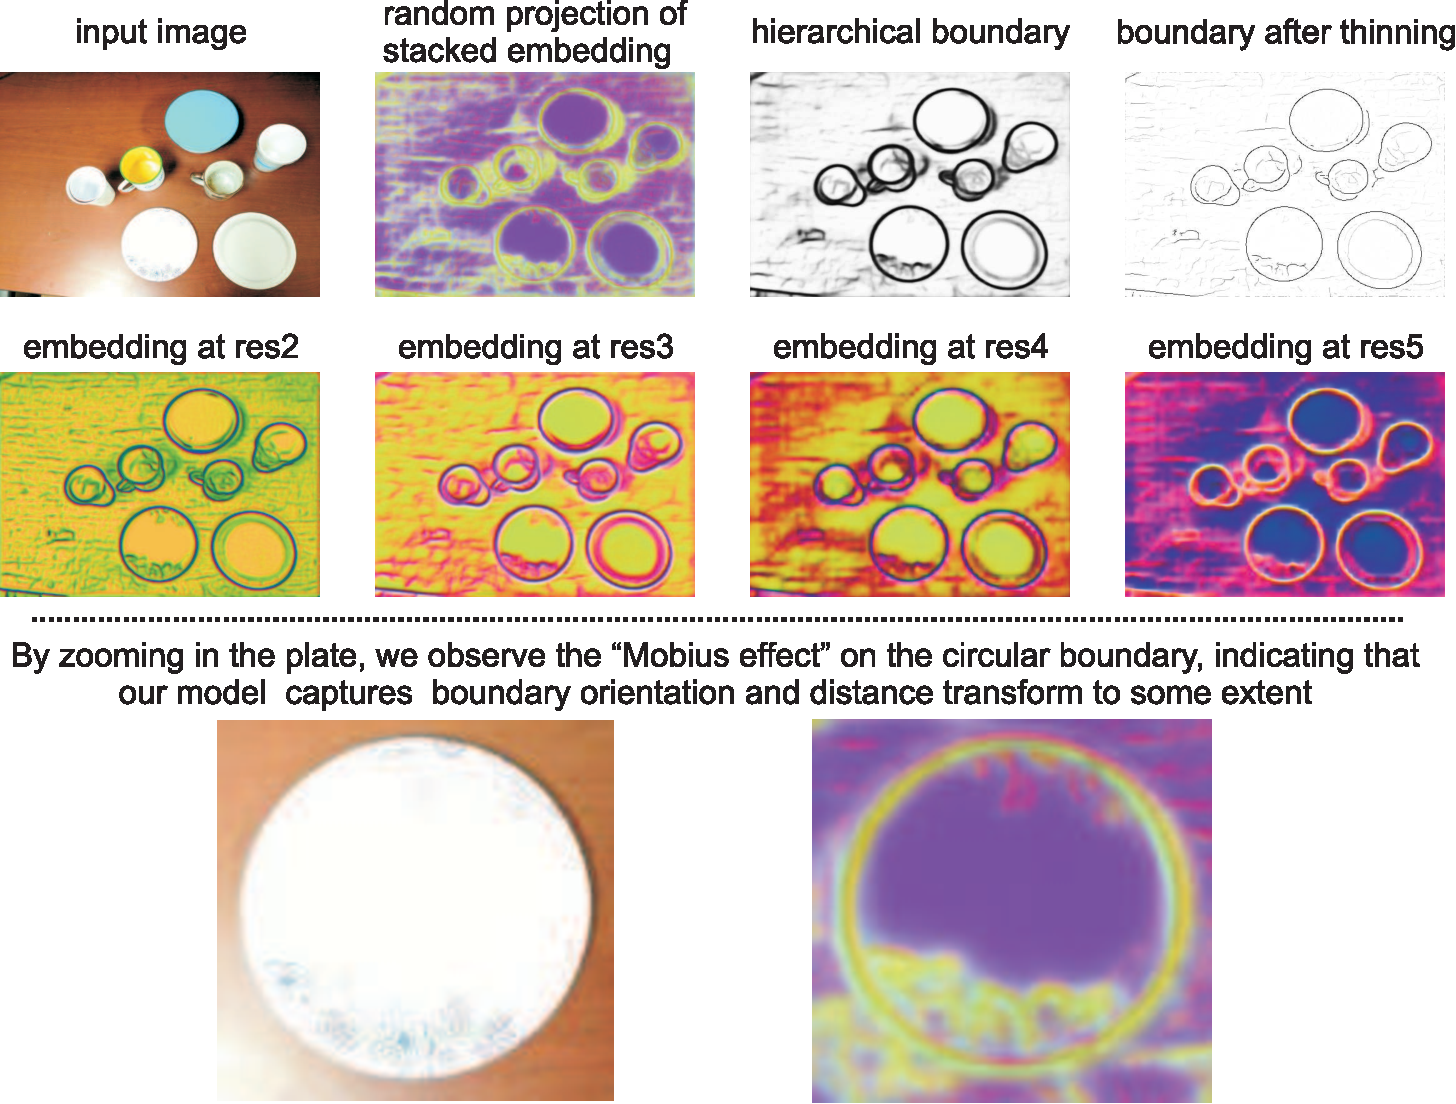
\includegraphics[width=0.7\linewidth]{demo_test_boundary}
   \vspace{-3mm}
   \caption{An image highlighting the structure of the embedding for an image
   with circular boundaries. We observe a ``Mobius effect'' where the embedding
   encodes both the orientation and distance to the boundary.}
\label{fig:demo_test_boundary}
\end{figure*}

\begin{figure*}[t]
\centering
   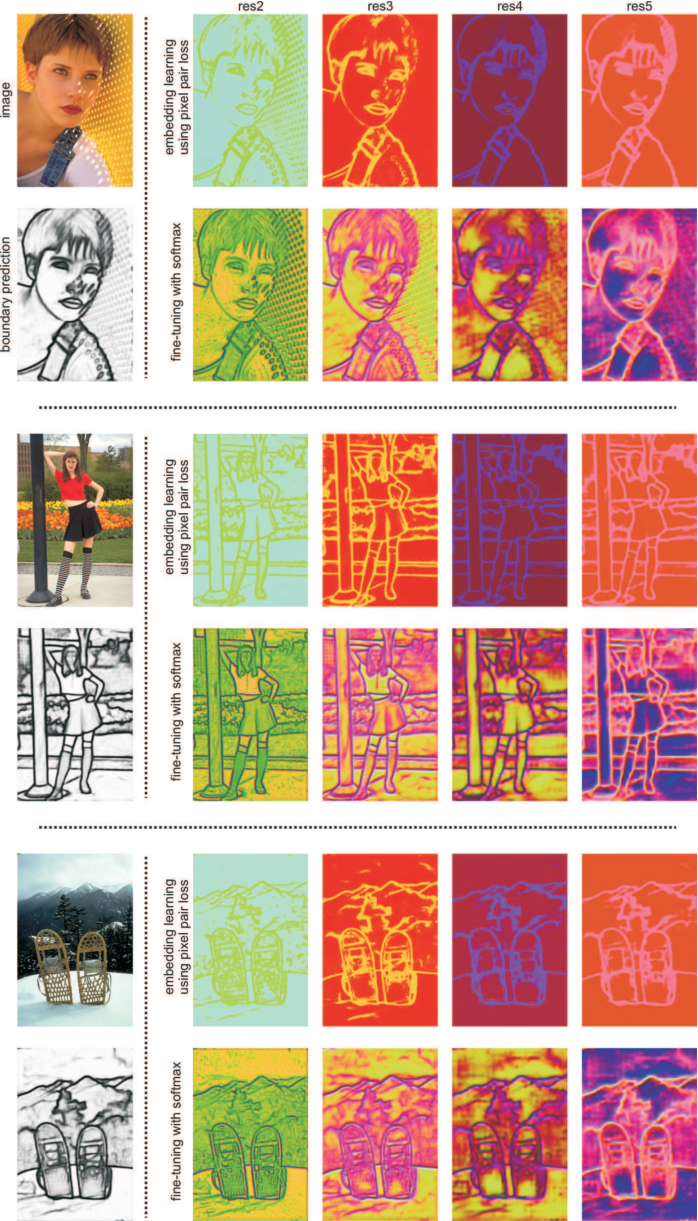
\includegraphics[width=0.7\linewidth]{boundary_show_appendix_part1_lowRes}
   \vspace{-3mm}
   \caption{Visualization for boundary detection (part-$1/5$).
   Images are randomly selected from BSDS500 test set.  For each image, we show
   the embedding vectors  at different layers from the model before and after
   fine-tuning using logistic loss.  We can see that the boundary embedding
   vectors after fine-tuning not only highlights the boundary pixels, but also
   captures to some extent the edge orientation and distance from the colors
   conveyed.
   }
\label{fig:boundary_show_appendix_part1}
\end{figure*}

%\begin{figure*}[t]
%\centering
%   \includegraphics[width=0.7\linewidth]{boundary_show_appendix_part2_lowRes}
%   \vspace{-3mm}
%   \caption{Visualization for boundary detection ($2/5$).
%   Images are randomly selected from BSDS500 test set.  For each image, we show
%   the embedding vectors  at different layers from the model before and after
%   fine-tuning using logistic loss.  We can see that the boundary embedding
%   vectors after fine-tuning not only highlights the boundary pixels, but also
%   captures to some extent the edge orientation and distance from the colors
%   conveyed.
%   }
%\label{fig:boundary_show_appendix_part2}
%\end{figure*}

\begin{figure*}[t]
\centering
   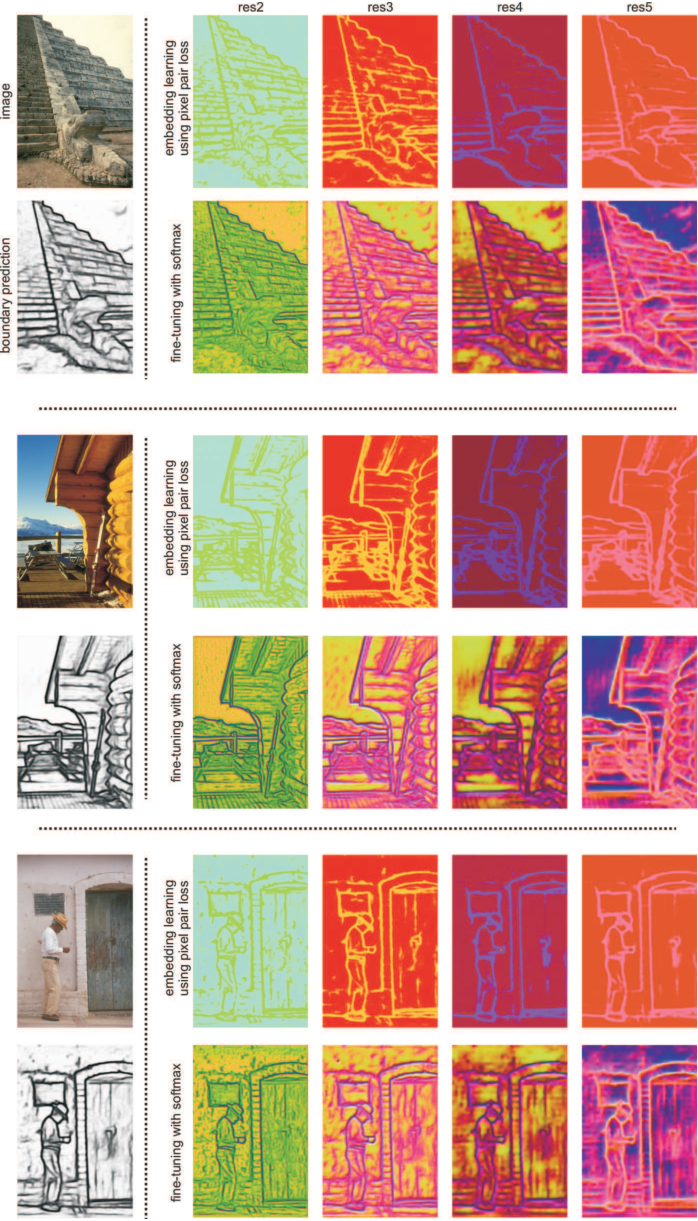
\includegraphics[width=0.7\linewidth]{boundary_show_appendix_part3_lowRes}
   \vspace{-3mm}
   \caption{Visualization for boundary detection ($3/5$).
   Images are randomly selected from BSDS500 test set.  For each image, we show
   the embedding vectors  at different layers from the model before and after
   fine-tuning using logistic loss.  We can see that the boundary embedding
   vectors after fine-tuning not only highlights the boundary pixels, but also
   captures to some extent the edge orientation and distance from the colors
   conveyed.
   }
\label{fig:boundary_show_appendix_part3}
\end{figure*}

\begin{figure*}[t]
\centering
   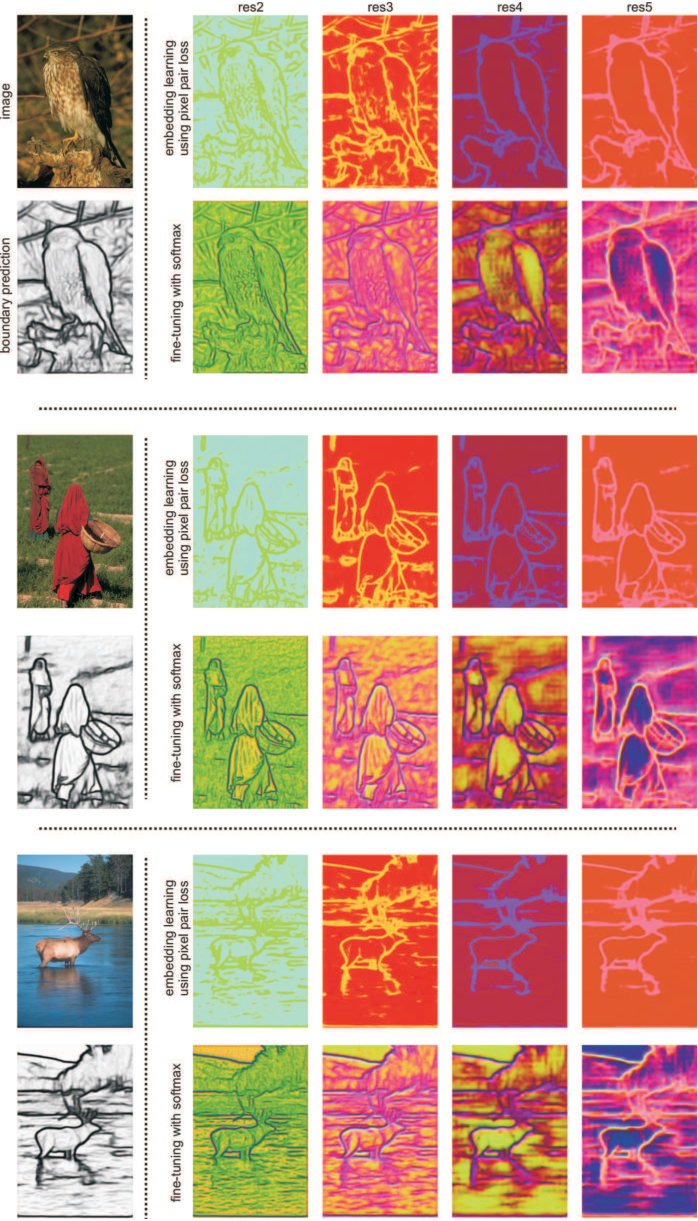
\includegraphics[width=0.7\linewidth]{boundary_show_appendix_part4_lowRes}
   \vspace{-3mm}
   \caption{Visualization for boundary detection ($4/5$).
   Images are randomly selected from BSDS500 test set.  For each image, we show
   the embedding vectors  at different layers from the model before and after
   fine-tuning using logistic loss.  We can see that the boundary embedding
   vectors after fine-tuning not only highlights the boundary pixels, but also
   captures to some extent the edge orientation and distance from the colors
   conveyed.
   }
\label{fig:boundary_show_appendix_part4}
\end{figure*}

\begin{figure*}[t]
\centering
   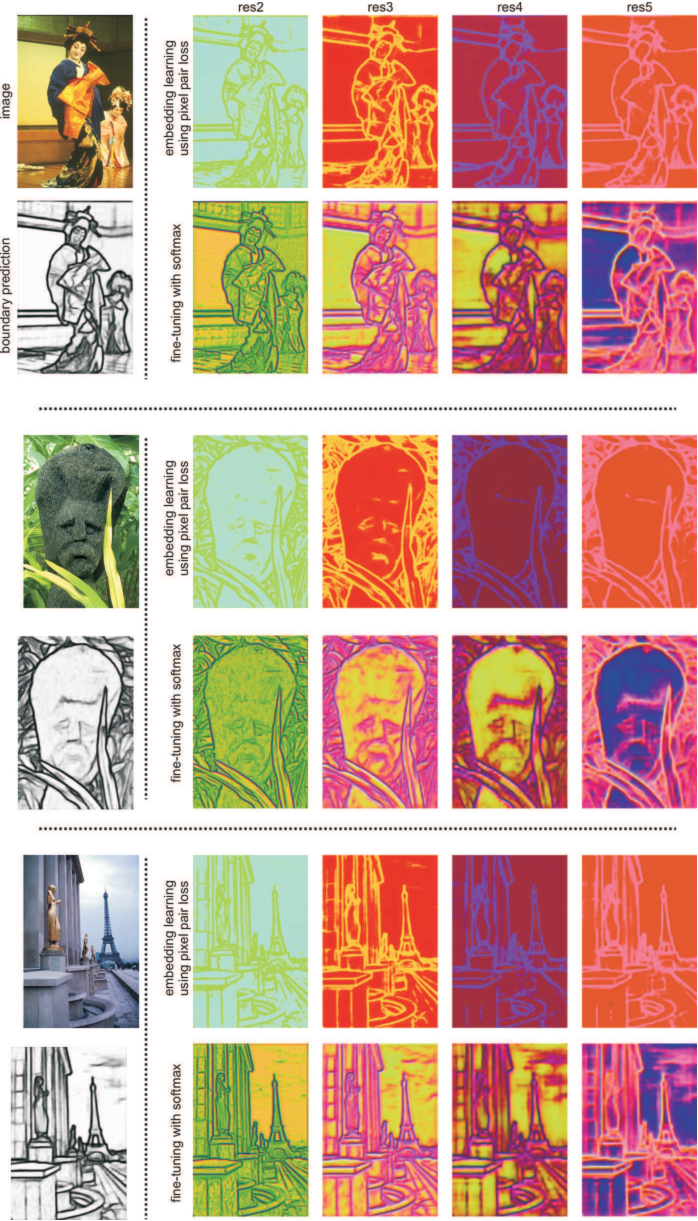
\includegraphics[width=0.7\linewidth]{boundary_show_appendix_part5_lowRes}
   \vspace{-3mm}
   \caption{Visualization for boundary detection ($5/5$).
   Images are randomly selected from BSDS500 test set.  For each image, we show
   the embedding vectors  at different layers from the model before and after
   fine-tuning using logistic loss.  We can see that the boundary embedding
   vectors after fine-tuning not only highlights the boundary pixels, but also
   captures to some extent the edge orientation and distance from the colors
   conveyed.
   }
\label{fig:boundary_show_appendix_part5}
\end{figure*}



\section{Additional Results on Instance-Level Semantic Segmentation}

We show more instance-level semantic segmentation results on PASCAL VOC 2012
dataset~\cite{everingham2010pascal} based on our model in Figure
\ref{fig:instSeg_show_part1}, \ref{fig:instSeg_show_part2} and
\ref{fig:instSeg_show_part3}.  
As we learn 64-dimensional embedding
(hyper-sphere) space, to visualize the results, we randomly generate three
matrices to project the embeddings to 3-dimension vectors to be treated as RGB
images.  Besides showing the randomly projected embedding results, we also
visualize the semantic segmentation results used to product instance-level
segmentation.  From these figures, we observe the embedding for background
pixels are consistent, as the backgrounds have almost the same color.
Moreover, we can see the embeddings (e.g. in
Figure~\ref{fig:instSeg_show_part1}, the horses in row-7 and row-13, and the
motorbike in row-14) are able to connect the disconnected regions belonging to
the same instance.  Dealing with disconnected regions of one instance is an
unsolved problem for many methods, e.g. \cite{bai2016deep,
kirillov2016instancecut}, yet our approach has no problem with this situation.

\begin{figure*}[t]
\centering
   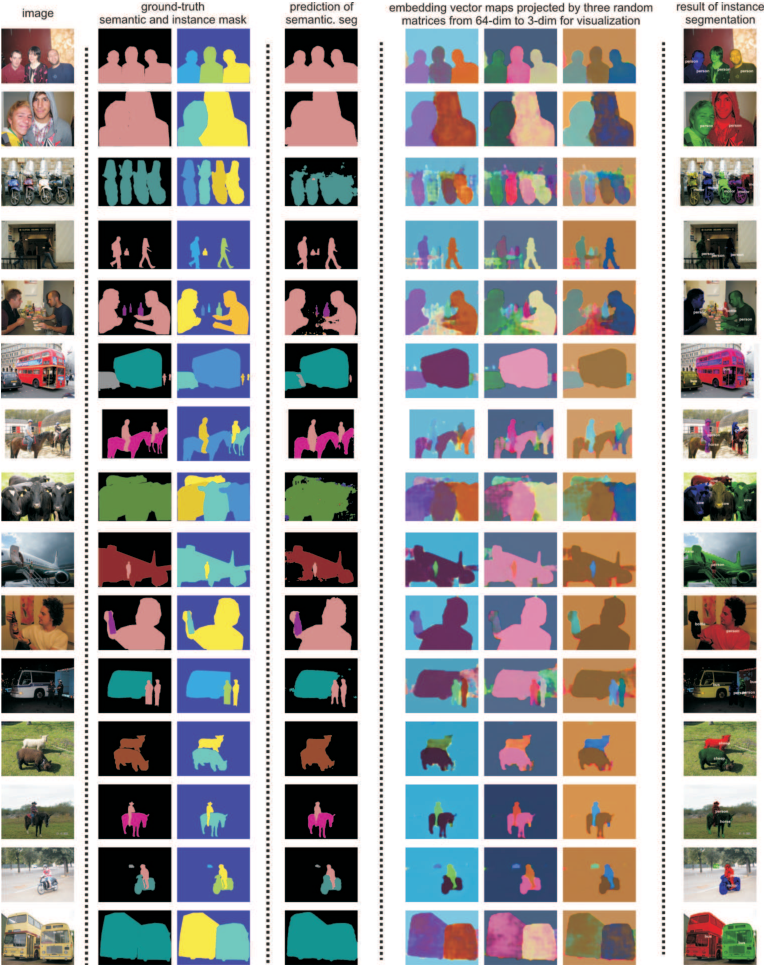
\includegraphics[width=0.95\linewidth]{instSeg_show_part1_lowRes}
   \caption{Visualization of generic and instance-level semantic segmentation
   with random projection of the embedding vectors (part-$1/3$).
   }
\label{fig:instSeg_show_part1}
\end{figure*}

\begin{figure*}[t]
\centering
   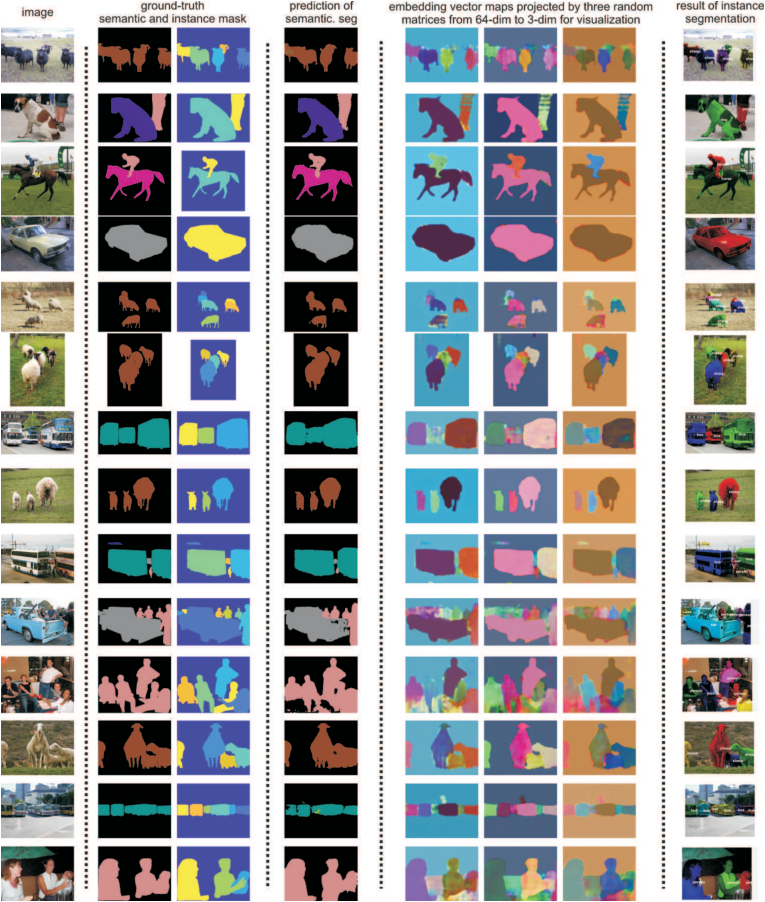
\includegraphics[width=0.95\linewidth]{instSeg_show_part2_lowRes}
   \caption{Visualization of generic and instance-level semantic segmentation
   with random projection of the embedding vectors (part-$2/3$).
   }
\label{fig:instSeg_show_part2}
\end{figure*}

\begin{figure*}[t]
\centering
   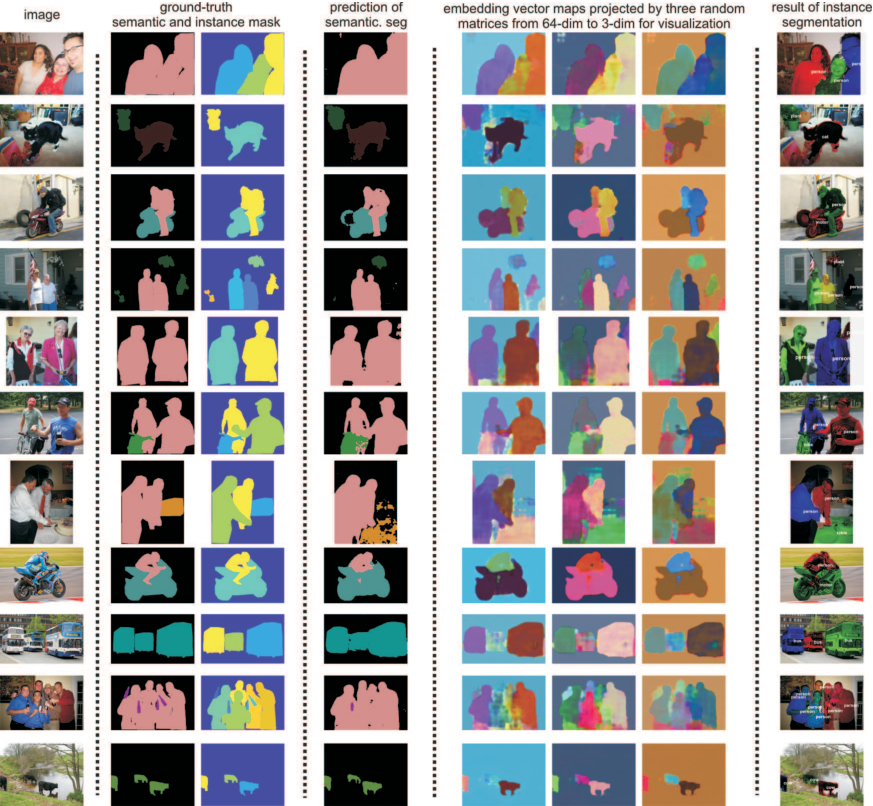
\includegraphics[width=0.95\linewidth]{instSeg_show_part3_lowRes}
   \caption{Visualization of generic and instance-level semantic segmentation
   with random projection of the embedding vectors (part-$3/3$).
   }
\label{fig:instSeg_show_part3}
\end{figure*}

